\chapter{Combined ABCD Rules and Dermoscopic Structures using Bayesian Network}

\section{Introduction}
In this chapter, we focus on the creation of a novel CAD framework that aims to automate the ABCD rules (Asymmetry, Border, Colour, and Dermoscopic structures) using SVM models and Bayesian fusion. To incorporate case-based reasoning, an Artificial Neural Network (ANN) is implemented to identify skin lesions with similar features.

This chapter proposes a CAD framework for the detection of melanoma using data extraction techniques to ensure the use of relevant features. The aim is to produce a transparent system focusing on providing information that would be useful to dermatologists and the impact of those features on the diagnosis. Metadata is included regarding age, gender, and anatomical location. Other features are asymmetry, border, colour, and dermoscopic structures. These are then combined using a Bayesian network. Case-based reasoning is also implemented to find skin lesions with similar clinical features.

\section{Background}
Automatic systems are being developed for the early detection of melanoma because it can take 10 years of experience for an accuracy of 86\%\cite{Morton1998}. Melanoma is one of the most aggressive forms of cancer that can remain dormant from anywhere between 6 months and 10 years before developing into metastatic melanoma, which becomes substantially more difficult to cure\cite{UK2019}. Problematically, clinicians who are not trained specifically to diagnose melanoma are usually the first to attempt it. Improving the accuracy of these clinicians should increase the overall accuracy of detecting melanoma. The early detection of melanoma followed by a biopsy is known to completely cure the disease\cite{mohammadpour2019}. Furthermore, melanoma develops from melanocytes that create skin pigmentation through the production of melanin, making a brown patch on the skin. Therefore, it has a clear indication of development on the surface of the skin. This means it is ideal for the creation of computer vision models for early detection.

For these reasons, there has been further interest in developing an automatic system for helping clinicians detect melanoma at its early stages. However, regardless of newer systems being developed they are still rarely implemented within clinical environments. This is largely due to systems producing parallel diagnosis, which does not explain how results were reached\cite{Lipton2018, Andre2017}. These techniques usually utilise Convolutional Neural Networks (CNN) because of their superior accuracy\cite{Wen2022}. There should be further explanations of the diagnosis for clinicians to understand and properly utilise within clinical environments. 

Newer machine learning models utilise explainable AI (XAI) to provide an explanation that provides further insight\cite{skar2017}. While these provide some indication of which area of the image has been used to train the algorithm they are still not tied directly to relevant clinical features. Furthermore, there appears to be a tradeoff between interpretability and model performance. Clinicians might not want to utilise models that are more interpretable, but less accurate. Furthermore, there has been some indication of models producing realistic but incorrect results\cite{Lipton2018}. In some scenarios, clinicians might be misled to falsely diagnose a skin lesion. Due to the high stakes involved when diagnosing melanoma, there should be highly accurate explanations and a track record of success before utilising them.

\section{Related Work}
In the design of CAD systems, two types of algorithms are employed. The initial type involves feature extraction, which is followed by individual classification methods. This process holds significant importance as it ensures the utilisation and visualisation of clinical features. The latter algorithm utilises the extracted features to classify different types of skin lesions. This method produces clinically relevant features that facilitate the diagnosis.

\subsection{Feature Extraction algorithms}
Ihab S. zaqout\cite{Zaqout2016} describes a technique using the centroid and rotation of the skin lesion using moments of inertia. The skin lesion is folded over vertically and horizontally subtracting the opposite halves. Pixels that cannot be subtracted are summed and compared with a threshold. If over the threshold the skin lesion is considered asymmetrical in that direction.

Reda Kasmi and Karim Mokrani\cite{Kasmi2016} describe a technique for comparing the colour distribution of the skin lesion by splitting the lesion into a 20 by 20 grid and comparing it against the colour of the perpendicular square using the 3D Euclidean distance. If over a threshold that square is considered asymmetrical. If more than half the lesions are over the threshold then the area is considered asymmetrical.

\subsection{Classification Methods}
A paper described by Javier Lopez, et al.\cite{Lopez-Labraca2018} describes a CAD system designed to provide clinicians with an enriched diagnosis. They utilise data extraction and classification techniques on dermoscopic structures, followed by combining the output of individual features using a Bayesian approach. This provides an indication of which features impact the diagnosis.

\section{Proposed Method}
The proposed CAD framework described in Figure\ref{model} automates the ABCD rules using statistical algorithms to extract features ($f$) from asymmetry, border, colour, and dermoscopic structures. Each feature has an associated SVM model trained using these extracted features. Next, Bayesian fusion, a probabilistic approach, combines multiple independent classifiers to diagnose melanoma. One benefit of Bayesian fusion is its higher accuracy in classifying skin lesions as compared to a standalone classifier\cite{Takruri2017}.  Javier López-Labraca, et al describe a similar method using dermoscopic structures, and colour\cite{Lopez-Labraca2018}. Other benefits are estimating the relevance of individual classifiers and classifying them with incomplete data, making it an interpretable and robust method. In addition, some feature extraction techniques generate graphics that might be suitable as an explanation for the diagnosis. Finally, the PH$^2$ dataset validates the rules, and once combined into a diagnosis, more extensive datasets, including ISIC 2019, measure its accuracy based on the diagnosis.

\begin{figure}
\begin{tikzpicture}[]

	%Image Acquisition
	\node (inp) [img] at (0, 3) {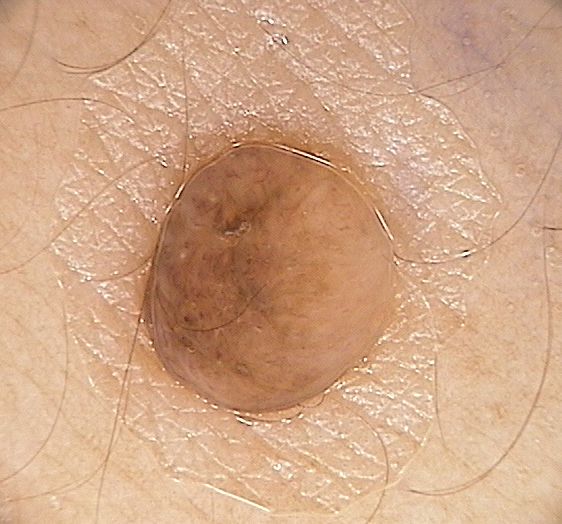
\includegraphics[scale=0.12]{images/lesion.png}};
	
	%Pre-processing
	\node (aug) [box, minimum height=1cm, node distance=3.6cm, right of=inp] {Augmentation};
	\node (seg) [box, minimum height=1cm, node distance=3.6cm, right of=aug] {Segmentation};
	
\node[draw=white] at ($(aug.north west)+(1.3,0.5)$) {\textbf{Pre-processing}};

\draw[thick, dotted] ($(aug.north west)+(-0.3,0.3)$) rectangle ($(seg.south east)+(0.3, -0.3)$);		

    %Feature extraction
    \node (asy) [box, right of=seg] at (0.0, 0.4) {Asymmetry};
    \node (bor) [box, right of=seg] at (0.0, -0.8) {Border};
    \node (col) [box, right of=seg] at (0.0, -2.0) {Colour};
    
    \node (asy2) [box, minimum width=1cm, right of=asy] {$f_a$};
	\node (bor2) [box, minimum width=1cm, right of=bor] {$f_b$};
    \node (col2) [box, minimum width=1cm, right of=col] {$f_c$};

		\node[draw=white] at ($(asy.north west)+(1.9,0.5)$) {\textbf{Feature Extraction}};    
    
    \draw[thick, dotted] ($(asy.north west)+(-0.3,0.3)$) rectangle ($(col2.south east)+(0.3, -0.3)$);
    
    %Classification
    \node (asy3) [box, right of=asy2] {SVM$_a$};
	\node (bor3) [box, right of=bor2] {SVM$_b$};
    \node (col3) [box, right of=col2] {SVM$_c$};

	\node[draw=white] at ($(asy3.north west)+(1.3,0.5)$) {\textbf{Classification}};    
    
    \node (fus) [box, minimum height=3cm, minimum width=1.7cm, text width=2cm] at (10.56, -0.8) {Bayesian \\ Fusion};
    
    \draw[thick, dotted] ($(asy3.north west)+(-0.3,0.3)$) rectangle ($(fus.south east)+(0.3, -0.3)$);
      
    \node (out) [box, right of=fus, node distance=2.7cm, minimum height=1.9cm, minimum width=1.9cm, text width=2cm] {Benign or \\ Malignant};
    
	\draw[->]
			(aug) edge (seg)
			(asy) edge (asy2)
			(bor) edge (bor2)  
			(col) edge (col2)  
			(asy2) edge (asy3)
			(bor2) edge (bor3)  
			(col2) edge (col3)  
			  
;
	\draw[->] (bor3)
	-|	($(fus.west)+(-0.5, 0)$)
 	|- (fus)
;

	\draw[-] (asy3)
	-|	($(bor3.east)+(0.5, 0)$)
;

	\draw[-] (col3)
	-| ($(fus.west)+(-0.5, 0)$)
;

 	\draw[->] (inp) edge (aug)
 			(asy2) edge (asy3)
			(bor2) edge (bor3)  
			(col2) edge (col3)  
 			(fus) edge (out)
 				(seg) -| ($(seg.east)+(0.7, 0)$)
 					  |- ($(seg.east)+(0, -1.2)$)
 					  -| ($(asy.west)+(-0.8, 0)$)
 					  |- (asy)
;

 	\draw[->] ($(asy.west)+(-0.8, 0)$) 
 		  |- (bor)
;

	\draw[->] ($(asy.west)+(-0.8, -1.2)$) 
 		  |- (col)
; 
    
\end{tikzpicture}
\caption{Proposed CAD framework describing the segmentation, feature extraction  and classification process.}\label{model}
\end{figure}

The ABCD rules, a set of criteria employed for the early detection of skin cancer, especially melanoma, are instrumental in guiding clinicians and individuals in assessing potentially suspicious skin lesions. The acronym "ABCD" stands for asymmetry, border irregularity, color variation, and diameter. Each element serves as a crucial parameter in evaluating the characteristics of moles or lesions on the skin. The objective of utilising this diagnostic procedure is to visualise important features that GPs need to support their diagnosis. Automating this process will instantiate trust when automating skin lesion identification within clinical environments. Another advantage would be the automatic labelling of skin lesions, making it easier for dermatologists to identify later.

The CAD framework in figure\ref{model} describes a model of pre-processing, feature extraction, and classification stages. After segmentation, statistical algorithms extract features ($f$), representing a different rule. Next, SVM models individually process the extracted features and combine them into a final result between benign and malignant using Bayesian fusion.

%Briefly cover the techniques, tested and proven in the previous chapter


%In the methods section you need to explain all the algorithms used in past tense in enough detail that they can be reproduced. Mention established methods.


\subsection{Feature Extraction Methods}
ABCD rules in this refer to the asymmetry, border irregularity, colour variation, and dermoscopic structures. Sometimes the D in ABCD rules refers to the diameter of the skin lesion, but it is often removed for dermocopic structures because images are taken at different distances making the measurement of diameter unreliable. Furthermore, the detection of dermoscopic structures provides valuable information in detecting the melanoma mimic called seborrhoeic keratosis (SK)\cite{Minagawa2017}. 



\subsubsection{Asymmetry}
%Asymmetry algorithm description
The approach for identifying asymmetry in this chapter is adapted from the work of Reda Kasmi and Karim Mokrani\cite{Kasmi2016}. In the original method, a bi-fold technique is employed to determine the centroid and rotation of the skin lesion, followed by image rotation. Subsequently, the image undergoes a conversion to LAB colorspace and is divided into a 20 by 20 grid by averaging color areas. The modified technique, however, utilizes superpixels from Simple Linear Iterative Clustering (SLIC) introduced by Achanta et al.\cite{Achanta2012}, with a compactness ($C$) set to 20.

Each color square is compared with others perpendicular to the centroid (with bi-fold) using the 3D Euclidean distance of the color (LAB). The resulting distance score is accumulated in an array, and if more than half exceed a threshold of 6, the lesion is classified as asymmetrical, contributing a TDS score of 1. This process is repeated at a 90-degree orientation, adding another TDS score if asymmetry is detected.

The data presented in Figure\ref{} illustrates that employing superpixels better supports the thresholding process compared to the original technique. The boxplot data represents the Euclidean distance, summed and divided by the number of positions.

%Super pixels diagram example showing different examples and 
\subsubsection{Colour}


%Colour analysis algorithm and diagram

\subsubsection{Dermoscopic Structures}

%Show dermoscopic structures pigment network

\subsection{Bayesian Fusion using Naive Bayes}
Bayesian fusion is a class of methods used to combine information from multiple sources taking into account uncertainty and probability distributions. This technique is frequently used for medical diagnosis for integrating data from various diagnostic tests to improve the accuracy of disease diagnosis\cite{}.

%Mention algorithms for combining the data 

\subsection{Case-Based reasoning using Artificial Neural Network (ANN)}



\section{Results}
%Simply mention what was found, but do not interpret the results or discuss their implementations. Present in logical order.
Two datasets were utilised to test the produced algorithms. The first is the PH2 dataset which includes asymmetry, colour, and dermoscopic structures.



\section{Discussion}


\section{Conclusion}